\documentclass[a4paper, 11pt]{article}
\usepackage{pdfsync}
\usepackage[pdftex]{color, graphicx}
\usepackage{verbatim}
\author{Xin Liu}
\title{TR-01: Using Template Recursion to Program Memory Hierarchy}
\begin{document}
\begin{abstract}
We introduce Vina, a template library designed to program memory hierarchy. We abstract hierarchical programming model within C++ language. Techniques in this report enable developers to 
write parallel programs while aware of specific machines and
memory hierarchies. To pursue high performance, Vina
emphases on the importance of separation of execution rules from
algorithms. In this form, programmers can focus on elaborating algorithm kernel and execution rules respectively, while C++ compiler takes responsibility to generate call graph
automatically, which credits from the powerful template mechanism.
\end{abstract}

\maketitle
\section{Background}
Computer system pursues high performance depending on two major approaches: parallelism and memory hierarchy.  Architects design and 
improve execution units to parallelize instruction processing, meanwhile, hierarchical storage systems shorten the latency of common load and
store operations based on temporal and spatial locality. A memory hierarchy consists of several levels of storage
with different speeds and sizes. Processor can obtain information from
closest level of hierarchy fastest. The lower levels of storage, however, are significantly cheaper so manufacturer can afford large volume.  In other word, you can build very fast storage, or very large storage, but no
storage that is both fast and large. This economic curse of memory hierarchy is never removed since the idea was born. Neither in
foreseeable future.

After decades of efforts, techniques to parallelize
instruction execution obtain huge success. Instruction pipeline is
implemented in almost all the modern microprocessors;  complex
predication and out of order execution mechanism significantly enhance performance of general purposed processors. 

On the other side, hierarchy approach is still waiting for essential breakthrough. The performance gap between processor and memory
is continuously increasing. In addition, the dominance of multicore system brings new problem -- horizontal communication among cores,
which further complicates exploitation of parallel machines.

Due to the fact mentioned above, the performance of programs are usually not limited in processor, but effective exploitation of
memory hierarchy, \textit{e.g.} careless use of spinlocks can easily suffocate bus bandwidth of SMP system with cache coherence protocol. Another example is that a programmer has to spend a lot of time to tune the granularity of an algorithm kernel in parallel program to maximize locality of cache or local storage. 

In order to compensate the speed difference of processor and memory, there is a trend to complicate memory programming.
Years after years, developers are used to perceived this thumb-rule: a couple of registers are managed by compiler, and remains of memory hierarchy are hardware's problem. However, the rule starts losing its power. CellBE ships the other 8 SIMD co-processors with a general purposed PowerPC. The most obvious difference is explicit DMA management between Virtual Memory and limited local storage only visible in co-processor respectively. Actually, it brings back the painstaking development
existed in the Neolithic age of computer system.  It is noteworthy that all 
x86\_64  quad-core processors (Nehalem and Barcelona)  ship bigger L3
cache to meet frequent communication among exponentially increasing cores. Larrabee follows this philosophy and will officially
assigned L2 cache the mission of communication in many cores scenario. Although it is handled by hardware, it is impossible to achieve ultimate performance without software developers' interference.
 
\subsection{Sequoia}
To exploit potentials of parallel machines, compiler community \cite{dragonbook2e} emphasizes on  the importance of tools. Developing compiler and new programming models might relief programmer from more and more complex memory hierarchy. Especially, some architectures do not support to control data allocation and movement explicitly. Therefore, they highly depend on language constructs and compiler optimization to express parallelism and generate effective instructions. The characteristic of GPU follows the description.

\cite{DBLP:conf/sc/FatahalianHKLHPERADH06} is good exploration and has demonstrated the idea of programming memory hierarchy. 

Firstly, Sequoia defines a programming model. It  targets execution environment as a tree of machines, which an individual machine owns storage and specific capability of computation.  The model  matches innovative architectures such as CellBE. It also works fine with traditional memory hierarchy with cache, in which case the computational capability of immediate nodes degenerate into task controller with only control and data movement instructions. Furthermore, the model can easily extend to the other abstracts such as SMT logical processors or Virtual Memory including magnetic disks.

Secondly, Sequoia is a customized programming language oriented to array. Working as a C extension, it abstracts computation-intensive function as a cluster of procedures, which is \emph{Task} in Sequoia's term. Sequoia programmers specify a group of rules for a task. The rules correspond to map sub-procedures to lower machines and optional reduce methods afterward. Sequoia compiler generates call graph according to the rules. Naturally, for multi-processor or multi-core architectures, Sequoia can be used to express parallelism in such a neat way.

However, Sequoia as a language extension is restrictive. The basic data structure is array, which obviously prefer to scientific computation. The language provides decent constructs though, it does not cover all of common parallel patterns such as pipeline or task queue. Task definition is confined within strict syntax, the flexibility is far away from parallelizing general programs.  In addition, Sequoia is actually a source-to-source compiler, using graph-based IR to transform and optimize program. If physical architecture is heterogeneous multi-core such as CellBE, it relies on different compilers for different targets. It is not easy to discover optimizing communication routes in that way. Much worse, because Sequoia depends on separating compilers to perform optimization, it is impossible to optimize data transfers when they need to inter-operate among compilers.
\subsection{PPL and TBB}
A lot of library-based solutions for concurrency emerge in recent. PPL (Parallel Pattern Library) is a template library shipping with Visual Studio 2010. It aims at task-parallelism and also provides generic containers and algorithms with concurrency supports. TBB(Thread Block Builder) has a plentiful of containers and execution rules. In TBB, entities including partitioner and scheduler in TBB are created in runtime. Definitely, runtimes in both PPL and TBB have to guarantee their data structures are thread-safe. We believe they are good at task-level parallelism or sophisticated concurrent situation on general purposed(GP) processors. For processors with massive ALUs, the benefits might not offset the expense. Even on GP processor, solution presenting in this report is orthogonal to PPL and TBB. We only exploit parallelism that can be determined in compile time. Developers feel free to resort to other runtime solutions.
\subsection{C++ Template}
Originally, C++ template mechanism is invented to supersede C Preprocessor. It is type-safe and could facilitate generic programming. People subsequently found the potential of template computation by chance. \cite{todd-temp} later proved that template itself is Turing-Completeness. Template computation is very similar to the form of functional languages. Fortunately, the power of them is really equivalent.

Beside role as it is designed,  template techniques have been applied to a plenty of innovative purposes. \cite{modernc++} associates it with design pattern and formulates policy-based programming diagram. The template is fundamental utility to implement policies. \cite{c++metaprog} describes template meta-programming in depth. It also introduces MPL(Meta-Programming Library), which helps programmers manipulate integral values and types in compile time. 
\section{Vina}
Vina derives the thoughts of Sequoia and uses modern template techniques to program memory hierarchy. It is a library consisting of basic containers and map classes to convenient programmers. Instead of dynamic containers such as std::vector, we implemented static length vector and 2-dimension matrix to simulate functionality of Sequoia. A transform class is \emph{meta function} which takes a function as input, generates modified version while keeping signature same. Essentially, transform class works as code generator that applies a series of rules and produces a call graphs internally. Current Vina is written based on Sequoia capability. In addition, to demonstrate our approach is easy to beyond it, we also implemented pipeline processing transformation. The following text is structured in this way. The remaining section describes rationale of library design and mechanisms of necessary techniques. Reader have to know basic template grammar and principles. Template meta-programming skill is not prerequisite but really helpful.  The next section entries implementation domain.  We emphasize on the separation of algorithm and execution rules, which we regard as critical point to obtains high performance on specific hardwares. [section 4] is evaluation and we will report experimental results  on x86\_64 multi-core architecture (and CellBE). Final section is conclusion and further work plan.
\subsection{Rationale}
Function is the basic unit of program. It is not uncommon  that most of time consumed by small subset of functions. For example, Imagine or graphics are processed within a group of algorithms, which are usually referred as  \emph{kernels} in multimedia applications. It is kernel that consumes most of computational resources and determines overall performance and  user experiences. We mainly focus on those algorithm kernels and present Vina as a library-based and architecture-oriented approach to optimize kernels.

Mathematically, a function is single-target binary relation. A kernel usually corresponds to a specific mathematical or engineering calculation, such as matrix multiplication or convolution. They are usually self-contained,\textit{i.e.}, seldom other function calls are found inside kernels. However, because of a large amount of arithmetic computation and tight loops, non-trivial programs expect very effective implementation of kernels. Programmers spend most of time to tune those zone. Techniques such as assembly to utilize clever instructions, inline or macro for activation reduction  and \textit{vector}-lization are common maneuvers. Although we still need these elaborates to guarantee high performance, Vina can help programmer to isolate kernels from execution, with architecture preferences.
\begin{figure}
\centering
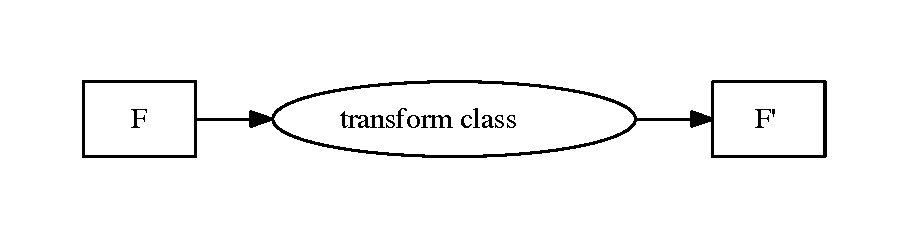
\includegraphics[width=0.9\textwidth]{map-class}
\caption{transform class}
\label{transform-class}
\end{figure}


A \emph{transform class(FT class)} is a template class which transforms a function to an isomorphic couterparter. As shown in Fig -~\ref{transform-class}, the right side of transform class is a function with exactly same type, but owns an Internal Call Graph(ICG) to complete the original computation. Traversal of internal call graph are called \emph{execution rules}. Without notice, other terms have same meanings of POSIX.  

Because transform classes are isomorphic, subscribers of a function can use or change them unconsciously, just like a \emph{policy}.  Replacing original function with ICG, we scrutinise both function body and target architectures.You might generate call graph using \textit{divide and conquer} or \textit{block}-lization. The strategies to produce call graph is not only for problem solving, but also aim at optimizing specific architectures. Modern computer systems contain complex memory hierarchy and ingenious layout of physical processing units(PEs). To effective utilize them, ICG and execution rule could correspond to target and express locality and parallelism in maximum. In Vina, they are not hardwired into program, alternatively, they are emitted in compile time. Developers program templates to control how call graph is built and traveled, C++ compiler is responsible for code generation using template system.

Matrix multiplication(MM) can be transformed into many sub-matrices multiplication and then reduce them. For large Matrices, cache usually can not accommodate them. Massive amount of cache misses will overwhelm the ALU time in many RISC processors when absent of out of order.  A call graph could be generated according to the size of lowest level cache(LLC), moreover, it might aware of the presence of multi-cores. Fig-~\ref{mm-icg} depicts a matrix multiplication kernel. Execution rules recursively divide computation until one fits target's LLC. Note that the shadow region are multi-threaded zone. we assume the target has two core so pair-wise threads are spawned at leaf nodes. 

\begin{figure}
\centering
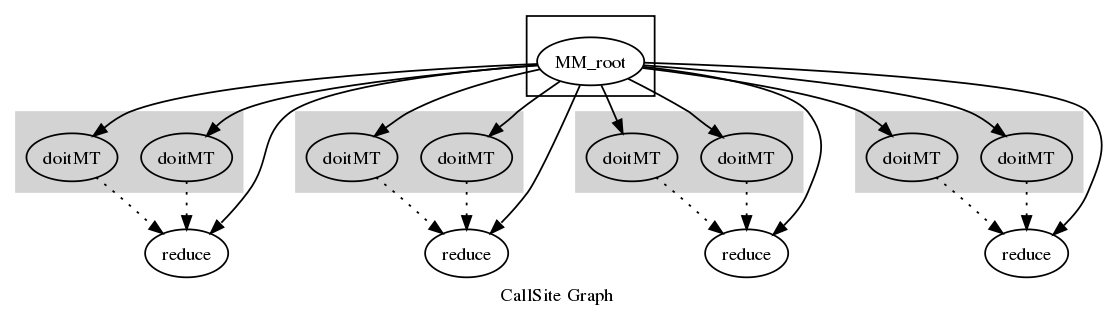
\includegraphics[width=\textwidth]{test_matrix}
\caption{MM internal call graph}
\label{mm-icg}
\end{figure}

\subsection{Mechanisms}
\subsubsection{predicate}
A \emph{predicate} is a meta-function which can be evaluated as a boolean value. In Vina, a predicate is a template class with only one boolean field. The qualifier of that field is static const. The initializer is an const expression. A predicate prefixes with 'p' as an indicator like lisp convention. Evaluation of its static field happens when the predicate is instantiating. The result of a predicate can be used as template arguments.
List - \textbf{1} is a predicate used in Matrix Multiplication. Give the type and the dimensions, this predicate estimates the need of storage. CACHE\_LL\_SIZE is the size of lowest level cache for target. The predicate roughly measures the computation scale and determines whether LLC can accommodate it.\\
\makebox[\textwidth]{\hrulefill}
\begin{verbatim}
template <class T, int SIZE_A, int SIZE_B, int SIZE_C>
struct p_lt_cache_ll {
  enum {CACHE_LL_SIZE = 4096*1024};
  const static bool value = ((SIZE_A * SIZE_B 
      + SIZE_A * SIZE_C + SIZE_B * SIZE_C) 
      * sizeof(T) ) <= CACHE_LL_SIZE;
};
or more modern style:
template <class T, int SIZE_A, int SIZE_B, int SIZE_C>
struct p_lt_cache_ll : boost::mpl::bool_<((SIZE_A * SIZE_B 
      + SIZE_A * SIZE_C + SIZE_B * SIZE_C) 
      * sizeof(T)) <= (4096*1024);>
{};
\end{verbatim}
\makebox[\textwidth]{\hrulefill}
\begin{center}
List - 1 : predicate lt\_cache\_ll
\label{code-pred}
\end{center}

\subsubsection{sentinel}
A \emph{sentinel} is template non-type parameter of transform class, with default initializer of a predicate. When template is instantiating, sentinels are evaluated. Usually, it is not intended to be assigned by external users. Because C++ lacks of invisible template parameter, we put sentinels to the end of template parameter list, and decorate them with mangled names. User provides predicates explicitly, but simply ignores sentinel. 

A predicate determines whether a specific of requirement has been satisfied. Sentinel is responsible for changing generation strategy when predicate becomes true. This is very similar with the branch instructions in traditional program. Template specialization in C++ can achieve this goal. The most common use of sentinel is as an indicator of leaf node. Presumably, leaf node exists on highest level of memory hierarchy, so leaf node should replace division procedure with concrete computation and finish call graph generation.
\subsubsection{view}
Generic programming can manipulate data while does not concern of specific types. This feature facilitates great flexibility of code reuse. A concept is a description of the requirements placed by a generic component.

Vina is also a generic library. Currently, it can manipulate two static data structure: Vector and 2-dimensional Matrix. They are the most common ADTs in multimedia domain. Because we reply on compile-time template recursion, the call graph is generated at that time and no code-generation capability remains in run time. Due to this limitation, we have to adapt static data structure. Sequoia also requires the size of array is resolved in compilation. This is essential limitation for languages lacking of dynamic code generation. Java and Python are pride of this ability, at the expense of runtime cost though.

In Vina, view is a concept. A view can refer to its underlying data structure which means it is modeled by containers. Furthermore, it can be tailored to support computation division. Fig-~\ref{vconcpt} depicts the concept of view and the relationship among them. For a concrete data-structure, it could induce two logic views: ReadView and WriteView. ReadView is restrictive because it is read-only. The dotted line indicates that explicit method is necessary to convert types. Solid line depicts auto-cast. Conversion toward a more restrictive type supports auto-cast because it is safe when sequential execution is guaranteed. 

It is worth noting that the shadow region is the other thread space. Only Multi-Threaded(MT) views are copyable across threads. The conversion from a MT View to a normal view is blocking operation. The underlying synchronization is signal. Signal is native facility for CellBE. Since shared memory system and POSIX environment do not have this communication among threads, we use conditional variable to simulate it. Reader should aware that view are not thread-safe and MT views act like ports of a harbor. They take responsibility of safe data-path. We omit the capacity of data access for MT views on purpose. User programmer can not bypass the synchronization if the lifetime of a view spans more than one thread.

The philosophy of design encourages streaming computation. A view represents a subset of pointing to aggregate data type. The operations on them have to be block-style to obtain high performance. The choice of signal instead of locks or transaction among MT views also reflects this preference.
\begin{figure}
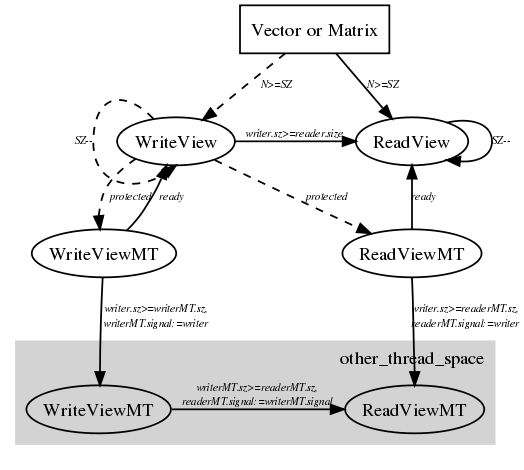
\includegraphics[width=\textwidth]{view_concept}
\caption{View Concept}
\label{vconcpt}
\end{figure}

\begin{comment}   %%%
\subsubsection{functor and bind}
Operator overload is a form of abstract mechanism. If member operator `()' is overloaded, a object could camouflage itself among normal functions. A object with this attribute is called \emph{functor}. Essentially, functor is an abstract of processing computation. However, computation would not start until code binds to \emph{environment}. Environment is a map from name to variable. Code is said to \emph{bind} an environment if all names are inquired in this environment. In terms of function, replacement parameters with arguments is also binding. Since functor abstracts \textit{processing} computation, if language support explicit binding, it is possible to postpone computation to anywhere. In a programming lifetime, anywhere means any temporal and spatial point after object is created.

Fortunately, C++ supports both functor and bind.
Deriving from boost, std::tr1::\emph{function} and std::tr1::\emph{bind} have been in C++ standardized literature[c++ tr1].

For transform class in Vina, normal function and functor are treated in uniform way. They are wrapped by a template class and travel generating call graph as template template parameter. In any node in ICG, wrapper can instantiate itself into functor, binding arguments and then start execution. Programmer should take responsibility for identifying optimal point and defining the way to execute it.
\end{comment}
\subsubsection{thread model}
\subsubsection{frame}
Frame consists of a set of template classes. A frame class represents a common prallel pattern. TF class associates with a specific parallel pattern by internal typedef or inheritance. 

vina::mappar partitions its task into \_K subtasks and then executes them independently.  
\begin{verbatim}
template <class Instance, int  _K,   bool _IsMT,
	  bool __SENTINEL__ >
struct mappar;
\end{verbatim}

A concrete TF class is provided as the first template parameter -- Instance, A couple of interfaces defines how to divide and compute as follows:
\begin{tabular}{|l|l|}
\hline
Instance::SubTask  &         SubTask of Instance \\
\hline
Instnace::Arg0 ... &         parameter types for primary task\\
\hline
Instance::Result   &         return type of primary task\\
\hline
Instance::\_pred    &         boolean value to determine it is leaf node\\
\hline
Instance::computation() &     return user define compuational function\\
\hline
Instance::computationMT() &    same as above, it is Multi-Thread version.\\
\hline
\end{tabular}
\\

It is worth noting that SubTask is just different instantiation of the same TF class, \textit{i.e.} the interface is recursive. The first parameter of SubTask can be addressed by Instance::SubTask::Arg0, etc.

The definition of vina::mappar is as follows:\\

\makebox[\textwidth]{\hrulefill}
\begin{verbatim}
struct mappar {
// ...
typedef mappar<typename Instance::SubTask, _K, _IsMT, 
	Instance::SubTask::_pred> _Tail;

static void doit(const typename Instance::Arg0& arg0, 
		     const typename Instance::Arg1& arg1, 
		     typename Instance::Result& result)
{
  for (int k=0; k < _K; ++k) {
      auto subArg0   = __aux::subview<typename Instance::Arg0, 
        arg0_dim::value, arg0_arithm::value>::sub_reader(arg0, k);
      auto subArg1   = __aux::subview<typename Instance::Arg1, 
        arg1_dim::value, arg1_arithm::value>::sub_reader(arg1, k);
      auto subResult = __aux::subview<typename Instance::Result, 
        result_dim::value, result_arithm::value>::sub_writer(result, k);

      _Tail::doit(subArg0, subArg1, subResult);
  }
}
// ...
};
\end{verbatim}
\makebox[\textwidth]{\hrulefill}
\begin{center}
List - 2 : mappar definition
\label{mappar-def}
\end{center}

Partition is tricky. We deploy template matafunctions to deal with exceptions. \textit{e.g.} if Arg0 is a scalar, \emph{\_\_aux::subview} will return itself or subset of ReadView othewise. The similar situation also happens when Frame classes find out Instance::Arg0 is the same as Instance::SubTask::Arg0 by arg0\_isomorph type in List-~\ref{bool-param}. In addtion, Frame has to be careful to handle Result type. If Result is WriteView, we has to clone it before binding to thread function, or multi-threaded environment may corrupt stack variables. On the otherside, we has to carefully obtain a reference if Result is a scalar, or the result value is invalid when function return. \emph{\_\_aux::ref} makes decision upon result\_arithm type, which is demonstrated in List-~\ref{leaf-spec}. We utilize template specialization and function overload to induce static information in compile-time, so there is no runtime-cost for code selection.

\makebox[\textwidth]{\hrulefill}
\begin{verbatim}
typedef mpl::bool_<std::tr1::is_arithmetic<typename
 Instance::Arg0>::value> arg0_arithm;
typedef mpl::bool_<std::tr1::is_same<typename Instance::Arg1,
 typename Instance::SubTask::Arg1>::value> arg0_isomorph;
...
typedef mpl::bool_<std::tr1::is_arithmetic<typename
 Instance::Result::value> result_arithm;
\end{verbatim}
\makebox[\textwidth]{\hrulefill}
\begin{center}
List - 3 : bool parameteres in mappar
\label{bool-param}
\end{center}

Finally, concret compuation is defined in leaf specializations. the last template parameter \_\_Sentinel\_\_ becames true, 
We partiailly specialize two versions: one is sequential, the other is multi-threaded.

\makebox[\textwidth]{\hrulefill}
\begin{verbatim}
  template<class Instance, int _K>
  struct mappar<Instance, _K, false, true>
  {
    static const int lookahead = 0;
    static void doit(const typename Instance::Arg0& arg0, 
		     const typename Instance::Arg1& arg1,
		     typename Instance::Result& result,
		     mt::barrier_t barrier = mt::null_barrier)
    {
      auto compF = Instance::computation();
      compF(arg0, arg1, boost::ref(result));
   }
  };
           
  template<class Instance, int _K>
  struct mappar<Instance, _K, true, true>
  {
    static const int lookahead = 0;
    static void doit(const typename Instance::Arg0& arg0, 
		     const typename Instance::Arg1& arg1,
		     typename Instance::Result& result,
		     mt::barrier_t barrier = mt::null_barrier)
    {
      auto compF = Instance::computationMT();
      mt::thread_t leaf(compF, arg0, arg1, 
          __aux::ref<typename Instance::Result>(result), 
          barrier);
      leaf.detach();
    }
  };
\end{verbatim}}
\makebox[\textwidth]{\hrulefill}
\begin{center}
List - 4 : Leaf specialization
\label{leaf-spec}
\end{center}

Besides of preceding \emph{mappar} , we has defines \emph{mapreduce} and their variants to support two dimentional data structure respectively. All of them has corresponding applications describing as follows.
\section{Case study and Evaluations}
\subsection{saxpy}
\subsection{dot\_prod}
\subsection{conv2d}
\subsection{mat\_mul}
\section{Conclusion}

\bibliographystyle{plain}
\bibliography{my}
\end{document}
